% questions.tex —— 2008 年·全国大纲卷Ⅱ·理科 · 题目内容片段（无答案）
% 由 tools/generate_projects.py 依来源总账自 2008/2008_数学真题_全国2理_试题.md 生成，勿手改（改源 MD 后重跑）


\gkpart{数学}

\begin{gktip}
\textbf{来源说明}：本题面依据固定源 PDF 两页 A3 题面逐题转录，原卷印刷页码 437–438。固定源不附答案，答案和解析均由本库独立复算。

\textbf{图形说明}：第 19 题的原卷图形关系重绘为 TikZ/PGFPlots 矢量图。图形标记所指的 PNG 不随仓库保存。
\end{gktip}

\gkpart{一、选择题}

\begin{question}
\gkti{1}设集合 $M=\{m\in\mathbb Z\mid-3<m<2\}$，$N=\{n\in\mathbb Z\mid-1\leqslant n\leqslant3\}$，则 $M\cap N=$\mbox{（　　）}

（A）$\{0,1\}$\quad（B）$\{-1,0,1\}$\quad（C）$\{0,1,2\}$\quad（D）$\{-1,0,1,2\}$

\end{question}
\begin{question}
\gkti{2}设 $a,b\in\mathbb R$ 且 $b\ne0$，若复数 $(a+b\mathrm i)^3$ 是实数，则\mbox{（　　）}

（A）$b^2=3a^2$\quad（B）$a^2=3b^2$\quad（C）$b^2=9a^2$\quad（D）$a^2=9b^2$

\end{question}
\begin{question}
\gkti{3}函数 $f(x)=\dfrac1x-x$ 的图象关于\mbox{（　　）}

（A）$y$ 轴对称\quad（B）直线 $y=-x$ 对称\quad（C）坐标原点对称\quad（D）直线 $y=x$ 对称

\end{question}
\begin{question}
\gkti{4}若 $x\in(e^{-1},1)$，$a=\ln x$，$b=2\ln x$，$c=\ln^3x$，则\mbox{（　　）}

（A）$a<b<c$\quad（B）$c<a<b$\quad（C）$b<a<c$\quad（D）$b<c<a$

\end{question}
\begin{question}
\gkti{5}设变量 $x,y$ 满足约束条件

\nopagebreak[4]
\[
\begin{cases}
y\geqslant x,\\
x+2y\leqslant2,\\
x\geqslant-2,
\end{cases}
\]

则 $z=x-3y$ 的最小值为\mbox{（　　）}

（A）$-2$\quad（B）$-4$\quad（C）$-6$\quad（D）$-8$

\end{question}
\begin{question}
\gkti{6}从 $20$ 名男同学、$10$ 名女同学中任选 $3$ 名参加体能测试，则选到的 $3$ 名同学中既有男同学又有女同学的概率为\mbox{（　　）}

（A）$\dfrac9{29}$\quad（B）$\dfrac{10}{29}$\quad（C）$\dfrac{19}{29}$\quad（D）$\dfrac{20}{29}$

\end{question}
\begin{question}
\gkti{7}$(1-\sqrt{x})^6(1+\sqrt{x})^4$ 的展开式中 $x$ 的系数是\mbox{（　　）}

（A）$-4$\quad（B）$-3$\quad（C）$3$\quad（D）$4$

\end{question}
\begin{question}
\gkti{8}若动直线 $x=a$ 与函数 $f(x)=\sin x$ 和 $g(x)=\cos x$ 的图象分别交于 $M\text{、}N$ 两点，则 $|MN|$ 的最大值为\mbox{（　　）}

（A）$1$\quad（B）$\sqrt2$\quad（C）$\sqrt3$\quad（D）$2$

\end{question}
\begin{question}
\gkti{9}设 $a>1$，则双曲线 $\dfrac{x^2}{a^2}-\dfrac{y^2}{(a+1)^2}=1$ 的离心率 $e$ 的取值范围是\mbox{（　　）}

（A）$(\sqrt2,2)$\quad（B）$(\sqrt2,\sqrt5)$\quad（C）$(2,\sqrt5)$\quad（D）$(2,\sqrt5]$

\end{question}
\begin{question}
\gkti{10}已知正四棱锥 $S-ABCD$ 的侧棱长与底面边长相等，$E$ 是 $SB$ 的中点，则 $AE\text{、}SD$ 所成的角的余弦值为\mbox{（　　）}

（A）$\dfrac13$\quad（B）$\dfrac{\sqrt2}{3}$\quad（C）$\dfrac{\sqrt3}{3}$\quad（D）$\dfrac23$

\end{question}
\begin{question}
\gkti{11}等腰三角形两腰所在直线的方程分别为 $x+y-2=0$ 与 $x-7y-4=0$，原点在等腰三角形的底边上，则底边所在直线的斜率为\mbox{（　　）}

（A）$3$\quad（B）$2$\quad（C）$-\dfrac13$\quad（D）$-\dfrac12$

\end{question}
\begin{question}
\gkti{12}已知球的半径为 $2$，相互垂直的两个平面分别截球面得两个圆。若两圆的公共弦长为 $2$，则两圆的圆心距等于\mbox{（　　）}

（A）$1$\quad（B）$\sqrt2$\quad（C）$\sqrt3$\quad（D）$2$

\end{question}
\gkpart{二、填空题}

\begin{question}
\gkti{13}设向量 $\boldsymbol a=(1,2)$，$\boldsymbol b=(2,3)$。若向量 $\lambda\boldsymbol a+\boldsymbol b$ 与向量 $\boldsymbol c=(-4,-7)$ 共线，则 $\lambda=$\gkblank{}。

\end{question}
\begin{question}
\gkti{14}设曲线 $y=e^{ax}$ 在点 $(0,1)$ 处的切线与直线 $x+2y+1=0$ 垂直，则 $a=$\gkblank{}。

\end{question}
\begin{question}
\gkti{15}已知 $F$ 是抛物线 $C:y^2=4x$ 的焦点，过 $F$ 且斜率为 $1$ 的直线交 $C$ 于 $A\text{、}B$ 两点。设 $|FA|>|FB|$，则 $|FA|$ 与 $|FB|$ 的比值等于\gkblank{}。

\end{question}
\begin{question}
\gkti{16}平面内的一个四边形为平行四边形的充要条件有多个，如两组对边分别平行。类似地，写出空间中的一个四棱柱为平行六面体的两个充要条件：充要条件①\gkblank{}；充要条件②\gkblank{}。（写出你认为正确的两个充要条件）

\end{question}
\gkpart{三、解答题}

\begin{question}
\gkti{17}在 $\triangle ABC$ 中，$\cos B=-\dfrac5{13}$，$\cos C=\dfrac45$。

（1） 求 $\sin A$ 的值；

（2） 设 $\triangle ABC$ 的面积 $S_{\triangle ABC}=\dfrac{33}{2}$，求 $BC$ 的长。

\end{question}
\begin{question}
\gkti{18}购买某种保险，每个投保人每年度向保险公司交纳保费 $a$ 元，若投保人在购买保险的一年度内出险，则可以获得 $10000$ 元的赔偿金。假定在一年度内有 $10000$ 人购买了这种保险，且各投保人是否出险相互独立。已知保险公司在一年度内至少支付赔偿金 $10000$ 元的概率为 $1-0.999^{10000}$。

（1） 求一投保人在一年度内出险的概率 $p$；

（2） 设保险公司开办该项险种业务除赔偿金外的成本为 $50000$ 元，为保证盈利的期望不小于 $0$，求每位投保人应交纳的最低保费。（单位：元）

\Needspace{0.4\textheight}
\end{question}
\begin{question}
\gkti{19}如图，正四棱柱 $ABCD-A_1B_1C_1D_1$ 中，$AA_1=2AB=4$，点 $E$ 在 $CC_1$ 上且 $C_1E=3EC$。
\nopagebreak[4]
\begin{center}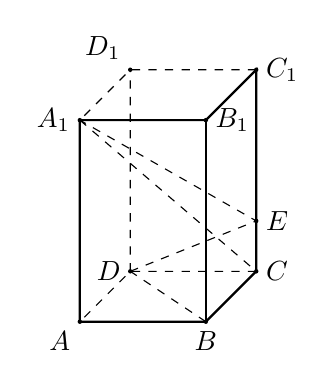
\begin{tikzpicture}[scale=.8,>=stealth]
\coordinate (A) at (0,0); \coordinate (B) at (2,0);
\coordinate (C) at (2.8,.8); \coordinate (D) at (.8,.8);
\coordinate (A1) at (0,3.2); \coordinate (B1) at (2,3.2);
\coordinate (C1) at (2.8,4); \coordinate (D1) at (.8,4);
\coordinate (E) at (2.8,1.6);
\draw[thick] (A)--(B)--(C)--(C1)--(B1)--(A1)--cycle;
\draw[dashed] (C)--(D)--(A) (C1)--(D1)--(A1) (D)--(D1);
\draw[thick] (B)--(B1) (C)--(C1);
\draw[dashed] (A1)--(C) (B)--(D) (D)--(E)--(A1);
\fill (A) circle (1pt) node[below left] {$A$};
\fill (B) circle (1pt) node[below] {$B$};
\fill (C) circle (1pt) node[right] {$C$};
\fill (D) circle (1pt) node[left] {$D$};
\fill (A1) circle (1pt) node[left] {$A_1$};
\fill (B1) circle (1pt) node[right] {$B_1$};
\fill (C1) circle (1pt) node[right] {$C_1$};
\fill (D1) circle (1pt) node[above left] {$D_1$};
\fill (E) circle (1pt) node[right] {$E$};
\end{tikzpicture}
\end{center}
\nopagebreak[4]
（1） 证明：$A_1C\perp$ 平面 $BED$；

（2） 求二面角 $A_1-DE-B$ 的大小。

\end{question}
\begin{question}
\gkti{20}设数列 $\{a_n\}$ 的前 $n$ 项和为 $S_n$。已知 $a_1=a$，$a_{n+1}=S_n+3^n$，$n\in\mathbb N^*$。

（1） 设 $b_n=S_n-3^n$，求数列 $\{b_n\}$ 的通项公式；

（2） 若 $a_{n+1}\geqslant a_n$，$n\in\mathbb N^*$，求 $a$ 的取值范围。

\end{question}
\begin{question}
\gkti{21}设椭圆中心在坐标原点，$A(2,0)$、$B(0,1)$ 是它的两个顶点，直线 $y=kx$（$k>0$）与 $AB$ 相交于点 $D$，与椭圆相交于 $E\text{、}F$ 两点。

（1） 若 $\overline{ED}=6\overline{DF}$，求 $k$ 的值；

（2） 求四边形 $AEBF$ 面积的最大值。

\end{question}
\begin{question}
\gkti{22}设函数 $f(x)=\dfrac{\sin x}{2+\cos x}$。

（1） 求 $f(x)$ 的单调区间；

（2） 如果对任何 $x\geqslant0$，都有 $f(x)\leqslant ax$，求 $a$ 的取值范围。

\end{question}